\documentclass{article}
\usepackage{amsmath,bm}
\usepackage{amssymb}
\usepackage{amsfonts}
\usepackage[usenames]{xcolor}
\usepackage{graphicx}
\usepackage{epsf}
\usepackage{hyperref}
\usepackage{enumitem}

% \usepackage[LGR,T1]{fontenc}
% \usepackage[sfdefault]{FiraSans}
% \usepackage[nomap]{FiraMono}
% \usepackage[var0,varqu]{zi4}
% \renewcommand{\rmdefault}{zi4}
%\renewcommand{\sfdefault}{zi4}

\usepackage{unicode}

% titlepage causes separate title page
% our latex is biased off 1in vertically and horizontally
\newtheorem{theorem}{Theorem}
\setlength{\topmargin}{0.1in}
\setlength{\oddsidemargin}{0in}
\setlength{\evensidemargin}{0in}
\setlength{\headheight}{0in}
\setlength{\headsep}{0in}
\setlength{\textheight}{9in}
\setlength{\textwidth}{6.5in}
% require that floats fill 90% of a page in order for that page to be
% ``float-only''
\renewcommand{\dblfloatpagefraction}{0.9}
\renewcommand{\floatpagefraction}{0.9}
\newenvironment{bibparagraph}{\begin{list}{}{ %
    \setlength{\labelsep}{-\leftmargin} %
    \setlength{\labelwidth}{0pt} %
    \setlength{\itemindent}{-\leftmargin} %
    \setlength{\listparindent}{0pt}}}{\end{list}}
\def\makefigure#1#2{\begin{figure}
\begin{center}
\input{#1}
\end{center}
\caption{#2}
\label{#1}
\end{figure}}

\def\limplies{\; \supset \;}
\def\land{\: \wedge \:}
\def\lor{\: \vee \:}
\def\iff{\; \equiv \;}
\def\lnot{\neg}
\def\lforall#1{\forall \: #1 \;}
\def\lexists#1{\exists \: #1 \;}
\def\glitch#1{{\tt #1}} % glitch on
%\def\glitch#1{} % glitch off
\def\comment#1{}
\def\pnil{[\;]}
\def\pif{\; \mbox{\tt :- } \;}
\def\tuple#1{$\langle #1\rangle$}
\def\mtuple#1{\langle #1\rangle}
\def\ceiling#1{\lceil #1\rceil}
\def\floor#1{\lfloor #1\rfloor}
\def\centerps#1{\begin{center}
\leavevmode
\epsfbox{#1}
\end{center}}
\def\argmax{\mathop{\rm argmax}}
\def\argmin{\mathop{\rm argmin}}
\def\grad{\nabla\!}
\def\celsius{^\circ\mbox{C}}
%\long\def\answer#1{}  % comment out for solutions
%\long\def\question#1{#1} % comment out for solutions
\long\def\answer#1{\color{green!10!blue!90!}{\sf \noindent #1}
\vspace{2ex}}  % comment in for solution
\long\def\question#1#2{\color{black}\rm \noindent {#1}.) #2 \par \vspace*{2ex}
} % comment in for solution
%\renewcommand{\labelenumi}{(\alph{enumi})}
%\newcommand{\mbx}{\mathbf{x}}
\newcommand{\mb}[1]{{\mathbf{#1}}}

\def\x{{\bf x}}
\def\w{{\bf w}}
\def\y{{\bf y}}

\usepackage{array}
\def\arraystretch{1.2}%


\begin{document}

{\small
Submitted by: {Oluwasegun Somefun}, somefuno@oregonstate.edu
}
{\Large
\begin{center}
  AI534 ---  IA3 Homework Report {Due Nov 14th 11:59pm, 2021}
\end{center}
}

\section{Introduction}

This report is on Perceptron and Kernels, with respect to the Implementation Assignment 3. 

\section{Part 1: Average Perceptron}
\question{a}{
  Comparing the training/validation accuracy curves of the average perceptron with those of the online perceptron, what do you observe? What are your explanation for the observation?
}
\answer{
\begin{figure}[!ht]
  \centering
  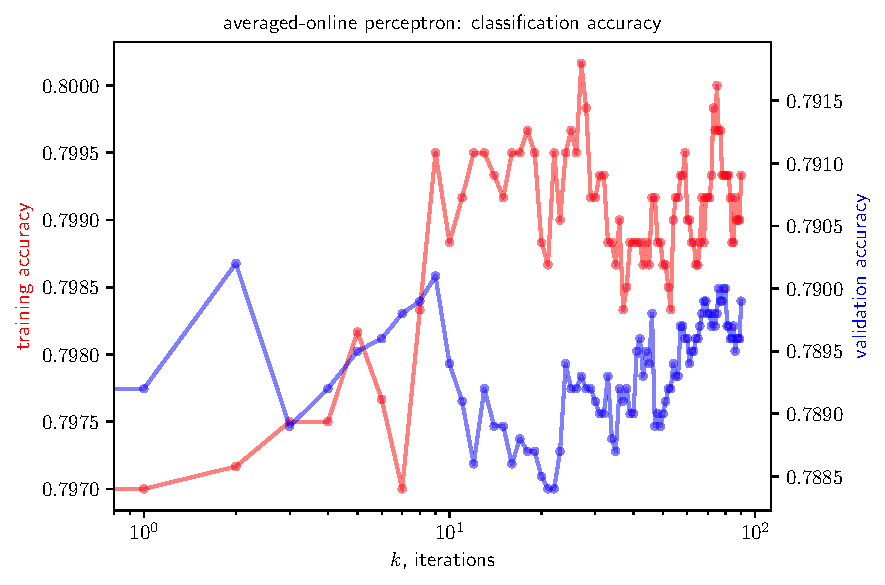
\includegraphics[width=0.5\linewidth]{figs/P1averaged-online_perceptron_plt.pdf}
  \caption{ Averaged-Online Perceptron: Training/validation class accuracy}\label{figa}
\end{figure}
\begin{figure}[!ht]
  \centering
  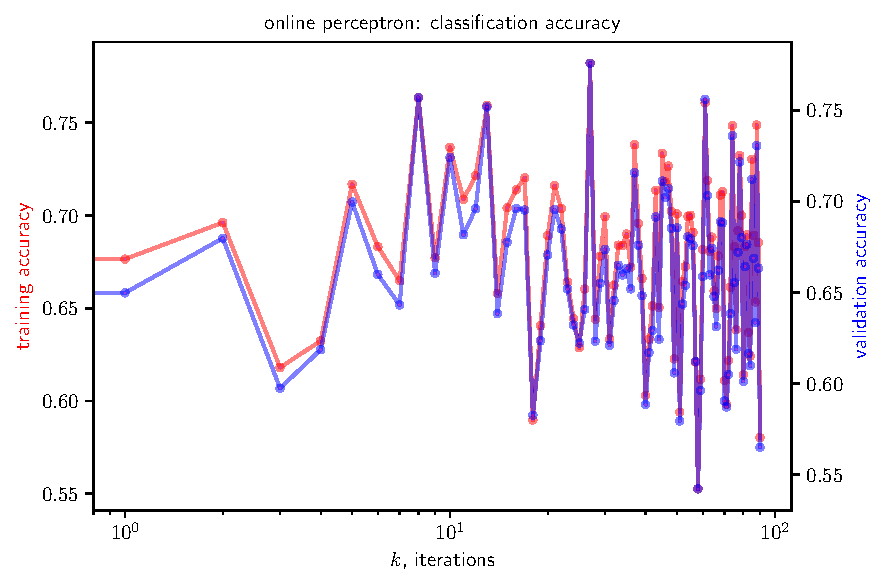
\includegraphics[width=0.5\linewidth]{figs/P1online_perceptron_plt.pdf}
  \caption{ Online Perceptron: Training/validation class accuracy}\label{figb}
\end{figure}
Generally, it can be observed that both accuracies are oscillatory as the iterations increase. For the averaged online perceptron, although the training accuracy generally increases, the validation accuracy generally oscillates around the same point. On the other hand, for the vanilla online perceptron, both the training accuracy and the validation accuracy generally oscillates around the same point. 
Overall, the averaged-online perceptron gives the best taining/validation accuracy over all iterations.

This makes sense, since the averaged perceptron uses a running weighted average of the weights, which are kept for testing, hence the weights in this form are more stable for testing predictions in online learning.

}

\question{b}{
  Which algorithm is more sensitive to the stopping point, (i.e., choosing different
  stopping point can lead to strong performance fluctuations) online or average perceptron? What
  are some practical implications of such sensitivity?
}
\answer{
The iteration number determining the potential early stopping point $k_e$ with respect to the class accuracies (training $A_t$ and validation $A_v$) for both algorithms are tabulated in Table~\ref{taba}. 

With respect to the iteration index $k$, it is clearly seen from Figures~\ref{figa}~and~\ref{figb}, that the vanilla online perceptron algorithm is more sensitive to the the chocie of a stopping point, since the accuracies are not stable, this can lead to undesired performance.
One practical implication of this is that the averaged perceptron should be used instead of the vanilla form, since it generalizes better to the data. However, the performance is still oscillatory and so, we still need to do early stopping to prevent overtraining the perceptron. Otherwise, this would lead to overfitting, in the sense that the algorithm starts learning the noise in the data.
  \begin{table}[!ht]
    \fontsize{10}{10} \centering \sf 
    \caption{Potential early-stopping point with respect to classification accuracy curves}
    \vspace{2ex}
    \begin{tabular}{|c|c|>{\bfseries}c|c|}
      \hline
      \textbf{Online Perceptron} & $A_t$ & $A_v$ & $k_e$ \\ \hline\hline
      Averaged         & 0.7993   & 0.7899   & 90  \\\hline
      Vanilla             & 0.7008    & 0.6855    & 50   \\\hline
    \end{tabular}
    \label{taba}
  \end{table}
% The resulting top five features with respect to their weight magnitude 
% are illustarated below with $\lambda^{*}=10^{-3}$, $\lambda_{+}=10^{-4}$ and
% $\lambda_{-}=10^{-2}$ in Table~\ref{tab1}. 
% Interestingly, in this range there is no much difference in the 
% selected top 5 features. However, as the value of $\lambda$ increases 
% outside this range, the top features, gradually begin to differ.
% \begin{table}[!ht]
%   \fontsize{10}{10} \centering \sf 
%   \caption{$\mathcal{L}_2$: Features (Top-5) with largest $|\mathbf{\omega}|$}
%   \vspace{2ex}
%   \begin{tabular}{|c|c|>{\bfseries}c|c|}
%     \hline
%     \textbf{Feature}            & $10^{-4}$ & $10^{-3}$ & $10^{-2}$ \\ \hline\hline
%     Previously\_Insured         & -3.2264   & -2.9705   & -2.0701   \\\hline
%     Vehicle\_Damage             & 2.2457    & 2.2035    & 1.9445    \\\hline
%     Policy\_Sales\_Channel\_160 & -1.8431   & -1.6671   & -1.3914   \\\hline
%     dummy                       & -1.0862   & -1.1732   & -0.9030   \\\hline
%     Policy\_Sales\_Channel\_152 & -0.8891   & -0.8424   & -0.6267   \\ \hline
%   \end{tabular}
%   \label{tab1}
% \end{table}
% This can be interpreted as automatic feature mapping during the regression process. 
% The optimization process automatically associates the most important features with larger weights
% relative to the other features.
}


\section{Part 2a: Online Perceptron with Polynomial Kernel}
\question{a}{
  As $p$ changes, do you see different trends for how training and validation accuracies
  vary with the number of training iteration? Do you see the risk of overtraining (i.e., when
  training for too many iterations leads to overfitting) for some p value? Please explain why this
  happens or does not happen for different p values?
}
\answer{
  Yes. As illustrated in Figures~\ref{fig2aa}~to~\ref{fig2ad}, as polynomial order $p\in{[1,2,3,4,5]}$ changes, the training and validation accuracies display different trends as the number of training iterations increases. 
  Particularly, the risk of overtraining almost linearly reduces as $p$ increases. With respect to the given fixed number of max-iterations, for $p=5$, the risk of overfitting is almost non-existing, as the class accuracies are celarly more stable and still increasing, compared to the other lower orders. 
  The problem in using polynomial kernels for mapping non-linearly 
  separable data to higher dimensions of linear separability is that selecting the polynomial order $p$ becomes a model selection problem or an hyperparameter that must be tuned to ensure a balance. This could be attributed to mean that $p=5$ gives the best bias-variance trade-off among the 5 values, and in this case it generalizes better to the validation data than the others.

  \begin{figure}[!ht]
    \centering
    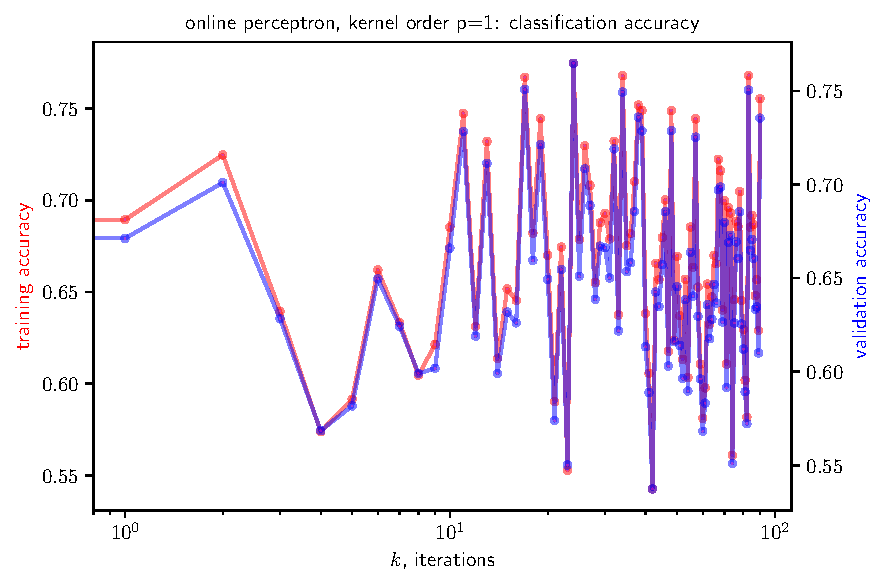
\includegraphics[width=0.45\linewidth]{figs/P2aonline_kernelperceptron_plt1.pdf}
    \caption{ Kernel Perceptron $p=1$: Training/validation class accuracy}\label{fig2aa}
  \end{figure}
  \begin{figure}[!ht]
    \centering
    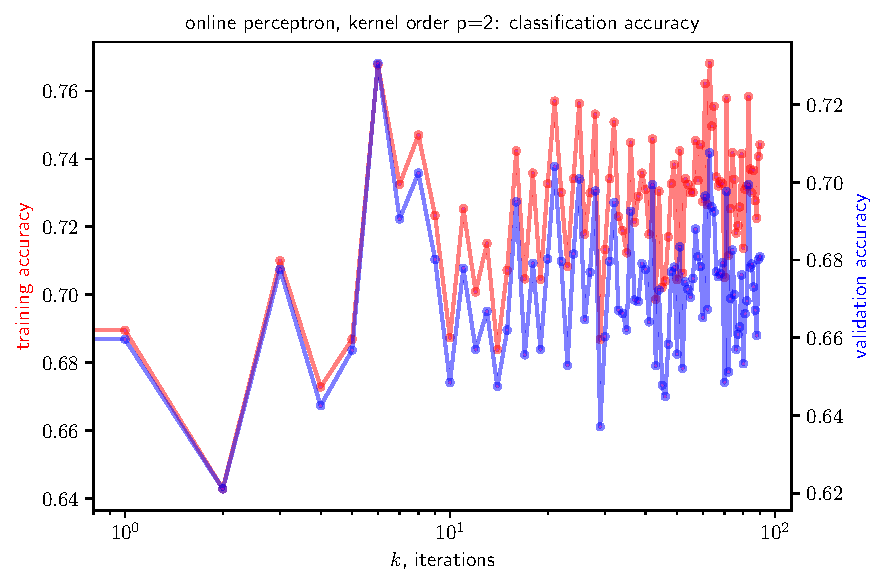
\includegraphics[width=0.45\linewidth]{figs/P2aonline_kernelperceptron_plt2.pdf}
    \caption{ Kernel Perceptron $p=2$: Training/validation class accuracy}\label{fig2ab}
  \end{figure}
  \begin{figure}[!ht]
    \centering
    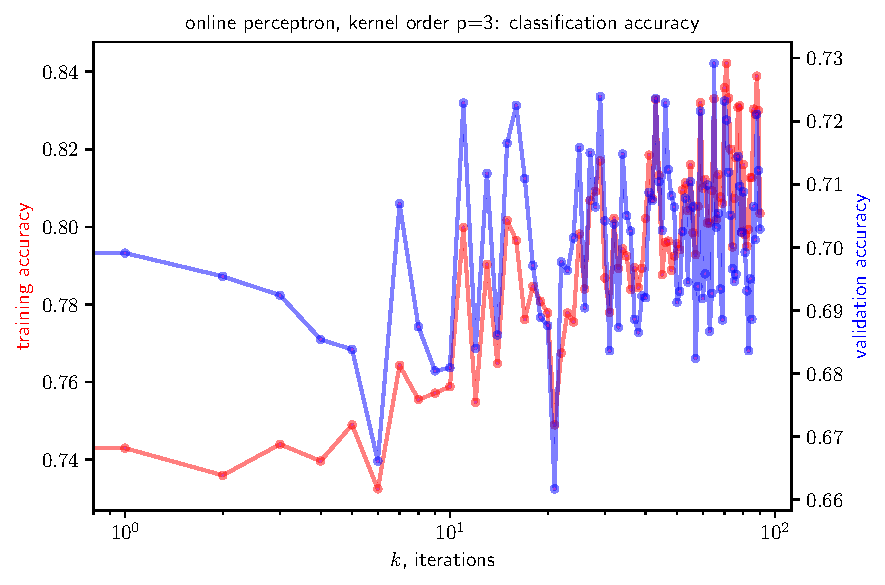
\includegraphics[width=0.45\linewidth]{figs/P2aonline_kernelperceptron_plt3.pdf}
    \caption{ Kernel Perceptron $p=3$: Training/validation class accuracy}\label{fig2ac}
  \end{figure}
  \begin{figure}[!ht]
    \centering
    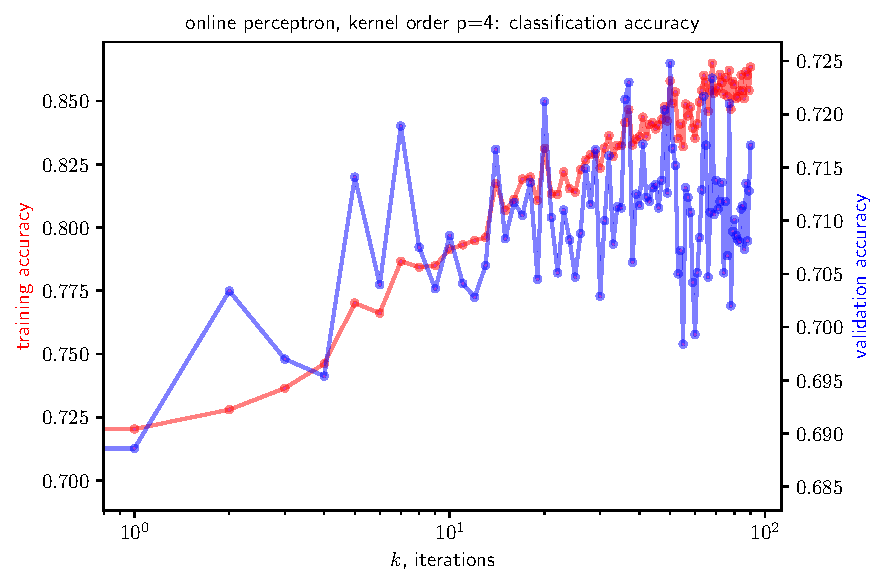
\includegraphics[width=0.45\linewidth]{figs/P2aonline_kernelperceptron_plt4.pdf}
    \caption{ Kernel Perceptron $p=4$: Training/validation class accuracy}\label{fig2ad}
  \end{figure}
  \begin{figure}[!ht]
    \centering
    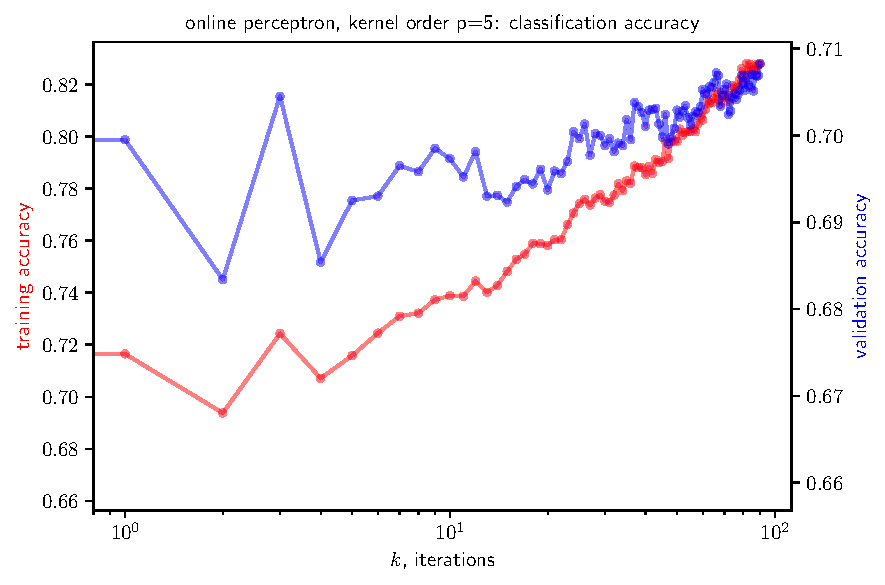
\includegraphics[width=0.45\linewidth]{figs/P2aonline_kernelperceptron_plt5.pdf}
    \caption{ Kernel Perceptron $p=5$: Training/validation class accuracy}\label{fig2ae}
  \end{figure}
}

\question{b}{
  Which value of $p$ produces the best validation accuracy? How do you think p is
  affecting the train and validation accuracy?
}
\answer{

  Reported in Table~\ref{tabb} are the best training and validation accuracy achieved for each p value (over all iterations).
  \begin{table}[!ht]
    \fontsize{10}{10} \centering \sf 
    \caption{Polynomial Kernel: best classification accuracy values for each order $p$}
    \vspace{2ex}
    \begin{tabular}{|c|c|>{\bfseries}c|c|}
      \hline
      \textbf{$p$} & $A_t$ & $A_v$ & $k_e$ \\ \hline\hline
      1         & 0.7553   & 0.7355  & 90  \\\hline
      2         & 0.7442   & 0.6809    & 90   \\\hline      3         & 0.8358   & 0.7232  & 70 \\\hline
      4         & 0.8580    & 0.7248    & 50   \\\hline
      5         & 0.8278   & 0.7083    & 90   \\\hline
    \end{tabular}
    \label{tabb}
  \end{table}
The best validation accuracy in terms of stability over all iterations is given by $p=5$. The increase in $p$ increases the capacity of the polynomial kernel for nonlinear spearability, hence an increase in $p$, should give increasingly better train and validation accuracy till some $p = p_e$ of diminishing returns, where the variance in the model increases (that is training accuracy increases, but validation accuracy does not)
}


\question{c}{
  What is the asymptotic runtime of your algorithm (in big $\mb{O}$ notation) in terms of the number of training examples $N$? Does your empirical runtime match up with the asymptotic analysis?
}
\answer{
\begin{figure}[!ht]
    \centering
    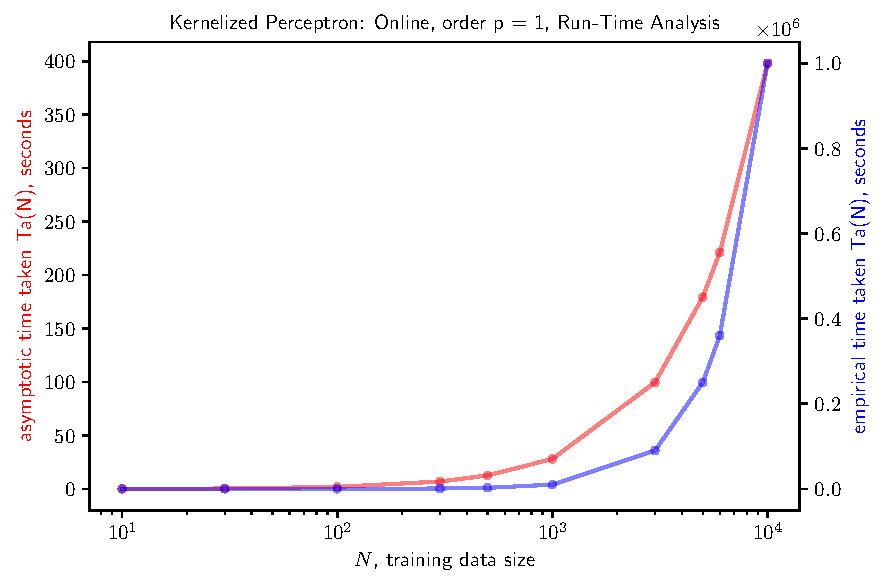
\includegraphics[width=0.55\linewidth]{figs/P2aconline_kernelperceptron_plt1.pdf}
    \caption{Algorithm Run-time: Kenelized Online Perceptron}\label{fig2ca}
\end{figure}
The empirical run-time and asymptotic run-time of the implemented kernelized online perceptron algorithm is shown in Figure~\ref{fig2ca}. It is clearly seen that the asymptotic run-time (in red) agrees with the empirical run-time (in blue).
The run-time data in Table~\ref{tab2ac}, the regressive fit approximates to a polynomial model:
$T_e(N) = 0.01\,N^{1.15}$ with a goodness of fit of $0.9744$.

\begin{table}[htbp]
	\centering
	\caption{Online Algorithm Run-Time Data for generating the empirical runtime model}
	\begin{tabular}{|c|c|}
		\hline
		$N$ & $T_e(N)$ in seconds \\ \hline\hline
	  10 & 352E-3 \\\hline
		30 & 596E-3 \\\hline
		50 & 1.65 \\\hline
		100 & 1.67 \\\hline
		300 & 4.21 \\\hline
		500 & 12.5 \\\hline
		1000 & 29.2 \\\hline
		3000 & 91 \\\hline
		5000 & 83 \\\hline
		6000 & 99 \\ \hline
	\end{tabular}
  \label{tab2ac}
\end{table}
The asymptotic run-time (in the worst-case) of the Kernelized Online Perceptron algorithm is quadratic, that is: $T_a (N) = \mb{O}(N^2)$.
This can be obtained by analysing the algorithm, which gives:
$T_a = kd N^2 + kN$, where $k$ is the fixed maximum iteration, $d$ is the fixed number of input features dimension. Clearly, we observe that the computation of the kernel matrix  which asymptotically is of quadratic polynomial order, contributes most to the algorithm's run-time in the worst-case.
}

\section{Part 2b: Batch Perceptron with Polynomial Kernel}
\question{a}{
  Comparing the curves for batch kernel perceptron with the ones acquired with the
  same $p$ value in part 2a, do you observe any differences? What are your explanations for them?

  Perceptron uses a fixed learning rate of 1 for the subgradient descent. What would be the impact if we use a different learning rate?

}
\answer{
  Yes, there is a significant difference, it seems the online kenrlized algorithm is more stable and higher for $p=5$ compared to its batch form which osciallates greatly. The reason for this is not clear, this may be due to the way the $\alpha$ in the kernelized batch form is being updated.
  \begin{figure}[!h]
    \centering
    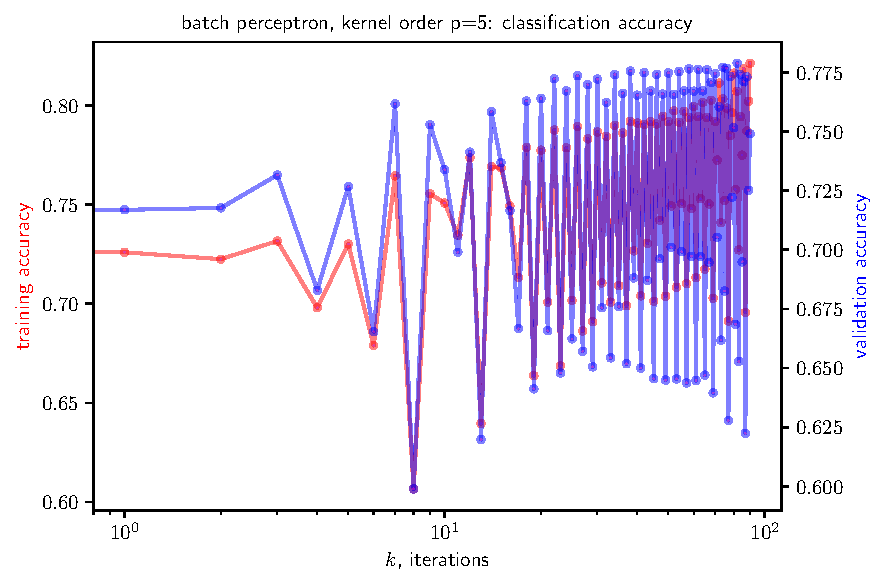
\includegraphics[width=0.55\linewidth]{figs/P2bbatch_kernelperceptron_plt5.pdf}
    \caption{Batch Kernel Perceptron $p=5$: Training/validation class accuracy}\label{fig2ca}
  \end{figure}

  The Perceptron uses a fixed learning rate of $1$ for the subgradient descent, which corresponds to a hinge-loss minimization with a margin-tradeoff penalty $C = 1$. This may indicate, in other words, that changing the learning-rate to another value, whether higher or smaller leads to a tradeoff between minimizing the maximum width of the linear decision boundary and minimizing the error.

}

\question{b}{
Provide the psudocode for your batch kernel perceptron algorithm. What is the asymptotic runtime of the batch kernel perceptron as a function of the number of training examples n? How does your empirical runtime match up with the asymptotic analysis? Do you observe a significant difference in runtime compared to the online algorithm? Provide an explanation for your observation.
}
\answer{
  \begin{figure}[!ht]
    \centering
    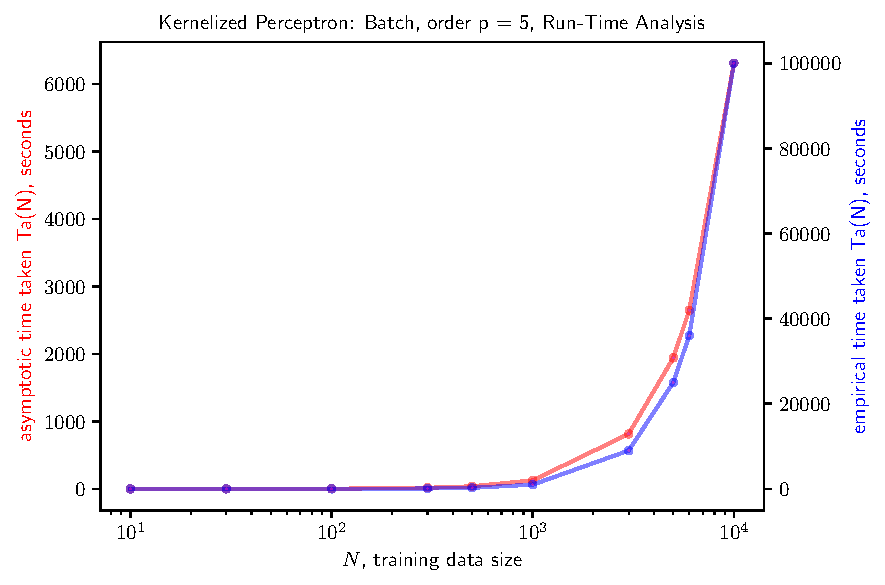
\includegraphics[width=0.45\linewidth]{figs/P2bcbatch_kernelperceptron_plt5.pdf}
    \caption{Algorithm Run-time: Kenelized Batch Perceptron}\label{fig2cb}
\end{figure}
The empirical run-time and asymptotic run-time of the implemented kernelized batch perceptron algorithm is shown in Figure~\ref{fig2cb}. It is clearly seen that the asymptotic run-time (in red) agrees with the empirical run-time (in blue).
The run-time data in Table~\ref{tab2bc}, the regressive fit approximates to a polynomial model:
$T_e(N) = 0.001\,N^{1.7}$ with a goodness of fit of $0.9738$.

\begin{table}[!th]
	\centering
	\caption{Batch Algorithm Run-Time Data for generating the empirical runtime model}
	\begin{tabular}{|c|c|}
		\hline
		$N$ & $T_e(N)$ in seconds \\ \hline\hline
	  10 & 415-3 \\\hline
		30 & 537E-3 \\\hline
		50 & 548E-3 \\\hline
		100 & 1.2 \\\hline
		300 & 2.58 \\\hline
		500 & 3.93 \\\hline
		1000 & 8.25 \\\hline
		3000 & 33 \\\hline
		5000 & 81 \\\hline
		6000 & 77 \\ \hline
	\end{tabular}
  \label{tab2bc}
\end{table}
The asymptotic run-time (in the worst-case) of the Kernelized Batch Perceptron algorithm is quadratic, that is: $T_a (N) = \mb{O}(N^2)$.
This can be obtained by analysing the algorithm, which gives:
$ T_a = kd N^2 + k$, where $k$ is the fixed maximum iteration, $d$ is the fixed number of input features dimension. Clearly, we observe that the computation of the kernel matrix which asymptotically is of quadratic polynomial order, contributes most to the algorithm's run-time in the worst-case.

Gnerally, although the empirical runtime, shows that the batch algorithm is slightly faster as the training data-size increases, there was no significant visible difference in the run-time compared to the kernelized online algorithm. This is due to the kernalization matrice being computed and accessed in both algorithms accounting for quadratic polynomial time in the worst-case.

The pseudocode for the Batch Kernel Perceptron is outlined in Table~\ref{tab2clast}
\begin{table}[!th]
	\centering
	\caption{Batch Kernel Perceptron Algorithm}
	\begin{tabular}{|c|l|}
		\hline
		Input & $\{(\x_i,y_i)\}_{1}^{N}$ (training data), $k$ (maximum iteration), kernel function $\kappa$\\ \hline 
    Output & $\alpha_1, \dots, \alpha_N$ \\ \hline\hline
	  1 & Initialize ${\{\alpha\}}_i^N \leftarrow 0$ for $i = 1,...,N$ \\\hline
    2 & for $i = 1,\dots,N, j = 1,\dots,N$ do\\
    3 & $K(i,j) = \kappa(\x_i,\x_j )$ \\
    4 & end\\
    5 & for $ t = 1$ to $k$ do\\
    6 & for each training example $\x_i$ do\\
    7 & $u_i \leftarrow \sum_{j=1}^N \alpha_j y_j K(i,j)$\\
    8 & end\\\hline
    9 & for each training example $\x_i$ do\\
    10 & if $ u_i y_i \le 0$ then\\
    11 & $\alpha_i \leftarrow  \alpha_i  + 1$\\
    12 & end\\
    13 & end\\
    14 & end\\\hline
	\end{tabular}
  \label{tab2clast}
\end{table}


}


\end{document}